\section{Results {\color{red}- Elicitation of words}}
\label{ResultsElicitation}
%
{\color{red} I dette afsnit skal der skrives om så det vores resultat der præsenteres er de 24 skalaer. 
Derudover skal opstillingen af resultaterne forbedres, så der ikke både er tabeller og punktopstillinger, for derved at gøre det mere overskueligt og få det til at fylde mindre.
Det skal kun være det vigtigste der står i dette afsnit}
Based on the 10 categories a variable can be elicited according to the criterion of a) being an influencing variable and b) the possibility of formulating the variable as a scale question. The field study was conducted on Danish speaking test subjects, and the variables are listed in both English and Danish. 

For each of the 10 categories the following statements are derived from the affinity diagram and will later serve as a basis for the potential scale. \textit{R} is short for robot.\\
%
\begin{itemize}
\item Appearance
\begin{enumerate}
  \item I think R's height is... (Jeg synes at R's højde er...)
  \item I think R is elegant... (Jeg synes R er elegant...)
  \item I think R looks human... (Jeg synes R ser menneskelig ud...)
  \item I like R's appearance... (Jeg kan godt lide R's udseende...)\\
\end{enumerate}
\item Trust in the robot 
\begin{enumerate}
  \item I feel safe around R (Jeg føler mig tryg ved R)
  \item I expect that R leads me to the chosen place (Jeg regner med at R følger mig hen til det sted jeg har valgt)
  \item R startled me (R gjorde mig forskrækket)\\
\end{enumerate}
\item Behaviour
\begin{enumerate}
  \item I think R's movements are... (Jeg synes R's bevægelser er...)
  \item I think R's speed is... (Jeg synes at R's hastighed er...)
  \item I think R is annoying... (Jeg synes R er irriterende...)
  \item I think R is alive... (Jeg synes R er levende...)
  \item I think R is intrusive... (Jeg synes R er anmassende...)\\
\end{enumerate}
\item Approach 
\begin{enumerate}
  \item I think R is welcoming (Jeg synes R er imødekommende)
  \item I think that R came too close to me (Jeg synes R kom for tæt på)
  \item I think that R was obstructive... (Jeg synes R stod i vejen)
  \item I was surprised by R's approach (Jeg blev overrasket over R's henvendelse)
  \item I thought that R was intimidating (Jeg synes R er intimiderende)\\
\end{enumerate}
\end{itemize}
%
When comparing the variables for HRI found in this study with variables for HRI from previous conducted studies on social robots \cite{PDF:ExploringInfluencingVariable}, \cite{PDF:SharingALifeHarvey}, \cite{PDF:InTheCompanyofRobots}, \cite{PDF:CloseButNotStuck}, \cite{PDF:TheImpactOfTraveler}, \cite{PDF:HumanRobotEmodiedInteraction}, \cite{PDF:RecommendationEffects}, variables such as distance, anthropomorphism, height, speed, movement, trust, and usefulness reoccur. New variables were found compared with previous mentioned studies. Under appearance such a variable is elegance. There was only found one new variable under trust which was if the robot startle you. According to behaviour the new variables found are how annoying and intrusive the robot was, and how calm or wild the movements of the robot were. Focusing on approach the new variables are how welcoming, obstructive, surprising, and intimidating the robot is perceived. In the following tables each individual scale question, noted with \textit{SQ}, is listed alongside the labels on the specific scale. If the scale does not contain a mid point it will be noted with \textit{-}, if it contains an unlabelled mid point it will be noted with \textit{No label}, whereas if the mid point is labelled the specific label is noted. 
%
\begin{table}[H]
	\centering
\caption{Scale labels for the robot's appearance}
	\label{tab:AppearanceScale} 
	\begin{tabular}{l|c|c|c}
		SQ     & Left label & Mid point & Right label \\\hline
		1   & \makecell{Too low \\(for lav)}  & \makecell{Appropriate \\(fin)} & \makecell{Too high \\(for høj)}        \\\hline
		2   & \makecell{Not at all elegant \\(slet ikke elegant)} & - & \makecell{Extremely elegant \\(ekstremt elegant)}         \\\hline
		3   & \makecell{Not at all human \\(slet ikke menneskelig)} & - & \makecell{Extremely human \\(ekstremt menneskelig)}         \\\hline
	 	4   & \makecell{Completely disagree \\(helt uenig)} & - & \makecell{Completely agree \\(helt enig)}         \\\hline
		5   & \makecell{Not at all startled \\(slet ikke forskrækket)} & -  & \makecell{Extremely startled \\(ekstremt forskrækket)}           
	\end{tabular}        
\end{table}
\noindent
%
%
\begin{table}[H]
	\centering
\caption{Scale labels regarding trust}
	\label{tab:TrustScale} 
	\begin{tabular}{l|c|c|c}
		SQ  & Left label & Mid point & Right label \\\hline
		1   & \makecell{Extremely unsafe\\ (ekstremt utryg)} & No label & \makecell{Extremely safe \\(ekstremt tryg)}          \\\hline
		2   & \makecell{Completely disagree \\(helt uenig)} & Neutral &\makecell{Completely agree \\(helt enig)} 
	\end{tabular}        
\end{table}
\noindent
%
%
\begin{table}[H]
	\centering
\caption{Scale labels for the robot's behaviour}
	\label{tab:BehaviorScale} 
	\begin{tabular}{l|c|c|c}
		SQ     & Left label & Mid point & Right label \\\hline
		1   & \makecell{Too calm \\(for rolige)} & No label & \makecell{Too wild \\(for vilde)}           \\\hline
		2   & \makecell{Too slow \\(for langsom)} & \makecell{Appropriate \\(fin)} & \makecell{Too fast \\(for hurtig)}   \\\hline
		3   & \makecell{Not at all annoying \\(slet ikke irriterende)} & - & \makecell{Extremely annoying \\(ekstremt irriterende)}          \\\hline
	 	4   & \makecell{Not at all alive \\(slet ikke levende)} & - & \makecell{Extremely alive \\(ekstremt levende)}         \\\hline
		5   & \makecell{Not at all intrusive \\(slet ikke anmassende)} & - & \makecell{Extremely intrusive \\(ekstremt anmassende)}             
	\end{tabular}
\end{table}
\noindent
%
%
\begin{table}[H]
	\centering
\caption{Scale labels for the robot's approach}
	\label{tab:ApproachScale} 
	\begin{tabular}{l|c|c|c}
		SQ     & Left label & Mid point & Right label \\\hline
		1   & \makecell{Very unwelcoming \\(meget afvisende)} & No label & \makecell{Very welcoming \\(meget imødekommende)}          \\\hline
		2   & \makecell{Too far \\(for langt væk)} & \makecell{Appropriate \\(tilpas)} & \makecell{Too close \\(for tæt på)}          \\\hline
		3   & \makecell{Not at all obstructive \\(slet ikke i vejen)}& -  & \makecell{Extremely obstructive \\(ekstremt i vejen)}  \\\hline
	 	4   & \makecell{Not at all surprised \\(slet ikke overrasket)} &  -  & \makecell{Extremely surprised \\(ekstremt overrasket)}       \\\hline
		5   & \makecell{Not at all intimidating \\(slet ikke intimiderende)} & - & \makecell{Extremely intimidating \\(ekstremt intimiderende)}           
	\end{tabular}
\end{table}
\noindent
%
The scale questions are presented on a \textit{Visual Analoge Scale} (VAS) with open anchor points, with or without mid point markers, and are either bi- or unipolar. If the scale is bipolar a mid point will be marked either with or without a label. Each scale consists of its own specific labels which are listed in \autoref{tab:AppearanceScale} for robot appearance, \autoref{tab:TrustScale} for robot trust,\autoref{tab:BehaviorScale} for robot behaviour, and \autoref{tab:ApproachScale} for robot approach. At the time of writing, the scales have not finally been developed but are expected to appear as shown on \autoref{fig:Height} for a bipolar scale with labelled mid point. 
%
\begin{figure}[H]
\centering

\includegraphics[width = 0.49\textwidth]{Figure/HeightHoejde} 
\caption{Example of a bipolar scale with a labeled mid point relevant for the scale question: \textit{I think R's height is...}}
\label{fig:Height}
\end{figure}
\noindent
% 
A bipolar scale without a label is expected to appear as shown on \autoref{fig:Calm}.  
%
\begin{figure}[H]
\centering
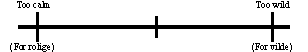
\includegraphics[width = 0.49\textwidth]{Figure/CalmWild} 
\caption{Example of a bipolar scale without a labeled mid point relevant for the scale question: \textit{I think R's movements are...}}
\label{fig:Calm}
\end{figure}
\noindent
%
An example of an unipolar scale as it is expected to appear is shown on \autoref{fig:HumanMenneskelig}.
%
\begin{figure}[H]
\centering
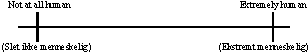
\includegraphics[width = 0.49\textwidth]{Figure/HumanMenneskelig} 
\caption{Example of an unipolar scale relevant for the scale question: \textit{I think R looks human}.}
\label{fig:HumanMenneskelig}
\end{figure}
\noindent
%
%I må gerne tjekke oversættelsen på SQ og labels, så sletter vi de danske SQ efterfølgende og skriver det vigtige
STARTER PÅ NY RESULTATER!\\
Based on the 10 categories a variable can be elicited according to the criterion of a) being an influencing variable and b) the possibility of formulating the variable as a scale question. The field study was conducted on Danish speaking test subjects, and thus the variables are listed in both English and Danish. In the following the 23 derived scales (noted S), along with the specific scale question (noted SQ), will be presented in corresponding order as presented for the test subjects in Experiment 2 and not according to the specific categories. 

The scale questions are all presented on a \textit{Visual Analoge Scale} (VAS) with closed anchor points and are either bi- or unipolar. If the scale is bipolar a mid point will be marked either with or without a label.\\
%
SQ1: How do think the screen on the robot reacted? (Hvordan synes du, at skærmen på robotten reagerede?)\\
SQ2: How did you experience the robot? (Hvordan oplevede du robotten?)\\
SQ3: How was it to use the robot? (Hvordan var det at bruge robotten?)\\
SQ4: How did you experience the robots movements? (Hvordan oplevede du robottens bevægelser?)\\
For each of the four scale questions the chosen labels are listed in \autoref{tab:ScalesPage1}.
%
\begin{table}[H]
	\centering
\caption{Scale labels PAGE 1}
	\label{tab:ScalesPage1} 
	\begin{tabular}{l|c|c|c}
		S     & Left label & Mid point & Right label \\\hline
		1   & \makecell{Extremely bad\\(Ekstremt dårligt)}  & No label & \makecell{Extremely well \\(Ekstremt godt)}        \\\hline
		2   & \makecell{Extremely unwelcoming \\(Ekstremt afvisende)} & No label & \makecell{Extremely welcoming \\(Ekstremt imødekommende)}         \\\hline
		3   & \makecell{Extremely difficult \\(Ekstremt svært)} & No label & \makecell{Extremely easy \\(Ekstremt nemt)}         \\\hline
	 	4   & \makecell{Extremely wild \\(Ekstremt vilde)} & No label & \makecell{Extremely calm \\(Ekstremt rolige)}               
	\end{tabular}        
\end{table}
\noindent
%
Each of the four scale questions mentioned above will be presented on scales similar to the one shown on \autoref{fig:TilpassetSkaermensReaktion}, which corresponds to SQ1. The remaining three SQs will be presented on the same type of scale with their corresponding labels listed in \autoref{tab:ScalesPage1}.  
%
\begin{figure}[H]
\centering

\includegraphics[width = 0.49\textwidth]{Figure/TilpassetSkaermensReaktion}
\setlength\abovecaptionskip{-1.2\baselineskip} 
\caption{Example of an bipolar scale relevant for the scale question: \textit{How do think the screen on the robot reacted?}.}
\label{fig:TilpassetSkaermensReaktion}
\end{figure}
\noindent
% 
SQ5: I think that the robot stoppede... (Jeg synes, at robotten stoppede...)\\
SQ6: I think that the robots speed is... (Jeg synes, at robottens hastighed er...)\\ 
SQ7: I think that the robots height is... (Jeg synes, at robottens højde er..)\\
For each of the three scale questions the chosen labels are listed in \autoref{tab:ScalesPage2}.  
%
\begin{table}[H]
	\centering
\caption{Scale labels PAGE 2}
	\label{tab:ScalesPage2} 
	\begin{tabular}{l|c|c|c}
		S     & Left label & Mid point & Right label \\\hline
		5   & \makecell{Way too close\\(Alt for tæt på)}  & No label & \makecell{Way too far \\(Alt for langt fra)}        \\\hline
		6   & \makecell{Way too slow\\(Alt for langsom)} & \makecell{Fine\\(Fin)} & \makecell{Way too fast \\(Alt for hurtig)}         \\\hline
		7   & \makecell{Way too low \\(Alt for lav)} & \makecell{Fine\\(Fin)} & \makecell{Way too high\\(Alt for høj)}                
	\end{tabular}        
\end{table}
\noindent
%
Each of the three scale questions mentioned above will be presented on scales similar to the one shown on \autoref{fig:TilpassetRStoppede}, which corresponds to SQ5. The remaining two SQs will be presented on the same type of scale with their corresponding labels and mid points listed in \autoref{tab:ScalesPage2}.  
%
\begin{figure}[H]
\centering
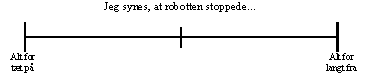
\includegraphics[width = 0.49\textwidth]{Figure/TilpassetRStoppede}
\setlength\abovecaptionskip{-1.2\baselineskip} 
\caption{Example of an bipolar scale relevant for the scale question: \textit{I think that the robot stopped...}}
\label{fig:TilpassetRStoppede}
\end{figure}
\noindent
% 
SQ8: I feel that the robot can help me (Jeg føler, at robotten kan hjælpe mig)\\
SQ9: I think that the robot was obstructing (Jeg synes, at robotten stod i vejen)\\
SQ10: I feel safe around the robot (Jeg føler mig tryg ved robotten)\\
SQ11: The robot startled me (Robotten gjorde mig forskrækket)\\
SQ12: I like to be served by the robot (Jeg kan godt lide at blive betjent af robotten)\\
SQ13: I counted on the robot to follow me to the location i chose (Jeg regnede med, at robotten fulgte mig hen til det sted jeg valgte)\\
Each of the six scale questions will be presented on the same type of scale with the same labels, as listed in \autoref{tab:ScalesPage3}. However, when presented for the subjects in Experiment 2 the scales will be presented three and three in the same order as presented above.   
%
\begin{table}[H]
	\centering
\caption{Scale labels for SQ8 to SQ13}
	\label{tab:ScalesPage3} 
	\begin{tabular}{l|c|c|c}
		S     & Left label & Mid point & Right label \\\hline
		8-13   & \makecell{Completely disagree\\(Helt uenig)}  & No label & \makecell{Completely agree\\(Helt enig)}                      
	\end{tabular}        
\end{table}
\noindent
%
The six aforementioned scales will be presented on scales similar to the one shown on \autoref{fig:TilpassetRobottenKanHjaelpe}, with their corresponding scale questions. 
%
\begin{figure}[H]
\centering
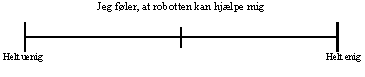
\includegraphics[width = 0.49\textwidth]{Figure/TilpassetRobottenKanHjaelpe}
\setlength\abovecaptionskip{-1.9\baselineskip} 
\caption{Example of an bipolar scale relevant for the scale question: \textit{I feel that the robot can help me}.}
\label{fig:TilpassetRobottenKanHjaelpe}
\end{figure}
\noindent
% 
SQ14: How personal did you experience the robots help? (Hvor personlig oplevede du robottens hjælp?)\\
SQ15: How surprised were you when the robot made contact? (Hvor overrasket blev du over robottens henvendelse?)\\
For each of the two scale questions the chosen labels are listed in \autoref{tab:ScalesPage5}. 
%
\begin{table}[H]
	\centering
\caption{Scale labels PAGE 5}
	\label{tab:ScalesPage5} 
	\begin{tabular}{l|c|c|c}
		S     & Left label & Mid point & Right label \\\hline
		14   & \makecell{Not at all personal\\(Slet ikke personlig)}  & - & \makecell{Extremely personal\\(Ekstremt personlig)}        \\\hline
		15   & \makecell{Not at all surprised\\(Slet ikke overrasket)} & - & \makecell{Extremely surprised \\(Ekstremt overrasket)}               
	\end{tabular}        
\end{table}
\noindent
%
The two scales listed in \autoref{tab:ScalesPage5} will be presented on an unipolar scale with corresponding labels. \autoref{fig:TilpassetPersonligHjaelp} shows the scale for SQ14. 
%
\begin{figure}[H]
\centering
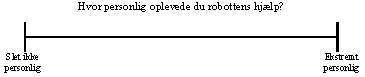
\includegraphics[width = 0.49\textwidth]{Figure/TilpassetPersonligHjaelp}
\setlength\abovecaptionskip{-1.2\baselineskip} 
\caption{Example of an bipolar scale relevant for the scale question: \textit{How personal did you experience the robots help?}.}
\label{fig:TilpassetPersonligHjaelp}
\end{figure}
\noindent
% 
The following eight scales, presented with two different scale questions, will also be presented on scales similar to the one shown on \autoref{fig:TilpassetPersonligHjaelp}, with their own labels. \\  
SQ16: What do you think about the robot? (Hvad synes du om robotten)\\
This scale question covers four different scales on which different parametres can be evaluated, these scales are presented with corresponding labels in \autoref{tab:ScalesPage6}. 
%
\begin{table}[H]
	\centering
\caption{Scale labels PAGE 6}
	\label{tab:ScalesPage6} 
	\begin{tabular}{l|c|c|c}
		S     & Left label & Mid point & Right label \\\hline
		16   & \makecell{Not at all annoying\\(Slet ikke irriterende)}  & - & \makecell{Extremely annoying \\(Ekstremt irriterende)}        \\\hline
		17   & \makecell{Not at all elegant \\(Slet ikke elegant)} & - & \makecell{Extremely elegant \\(Ekstremt elegant)}         \\\hline
		18   & \makecell{Not at all exciting\\(Slet ikke spændende)} & - & \makecell{Extremely exciting \\(Ekstremt spændende)}         \\\hline
	 	19   & \makecell{Not at all sweet \\(Slet ikke sød)} & - & \makecell{Extremely sweet \\(Ekstremt sød)}               
	\end{tabular}        
\end{table}
\noindent
%
SQ17: What do you else think about the robot? (Hvad synes du ellers om robotten?)\\
As with the aforementioned scale question, this scale question covers four different scales on which different parametres can be evaluated, these scales are presented with corresponding labels in \autoref{tab:ScalesPage7}  
%
\begin{table}[H]
	\centering
\caption{Scale labels PAGE 7}
	\label{tab:ScalesPage7} 
	\begin{tabular}{l|c|c|c}
		S    & Left label & Mid point & Right label \\\hline
		1   & \makecell{Not at all cool\\(Slet ikke sej)}  & - & \makecell{Extremely cool \\(Ekstremt sej)}        \\\hline
		2   & \makecell{Not at all intrusive \\(Slet ikke anmassende)} & - & \makecell{Extremely intrusive \\(Ekstremt anmassende)}         \\\hline
		3   & \makecell{Not at all funny\\(Slet ikke sjov)} & - & \makecell{Extremely funny \\(Ekstremt fun)}         \\\hline
	 	4   & \makecell{Not at all human \\(Slet ikke menneskelig)} & - & \makecell{Extremely human \\(Ekstremt menneskelig)}               
	\end{tabular}        
\end{table}
\noindent
%
Based on the affinity diagram a 24th parameter was derived, this parameter will not be presented along side the aforementioned scales but will be included in a seperat demographic page as it does not concern the robot. The parameter is formulated in the scale question: \textit{How happy are you with technology?}, which will be evaluated on a unipolar scale, similar to all other unipolar scales, with anchor points: \textit{Not at all happy} (slet ikke glad) and \textit{Extremely happy} (ekstremt glad).   




